

\chapter{TINJAUAN PUSTAKA}
\label{cha:2-TinjauanPustaka}

\section{Teorema Penaksiran Universal}
\label{sec:2-TeoremaPenaksiranUniversal}

Teorema penaksiran universal atau \textit{universal approximation theorem} menyatakan bahwa sebuah
model jaringan \textit{feed-forward} dapat membentuk fungsi apapun secara subjektif. Sebuah model
jaringan saraf tiruan dibentuk dari serangkaian lapisan yang didalamnya terdapat deretan sel saraf
atau \textit{neuron} dengan kuantitas tertentu. Semakin panjang rangkaian lapisan yang tersedia,
maka semakin banyak saraf yang tersedia sehingga dapat memetakan fungsi yang sulit.
Model jaringan yang memiliki banyak saraf dapat mempelajari pola-pola yang ada dari satu
domain ke domain lainnya~\cite{2016arXiv160100013G}.

Teorema penaksiran universal memiliki dua sifat yang dikategorikan berdasarkan pemanfaatannya dalam
melakukan pemelajaran mesin. Sifat pertama adalah suatu model jaringan saraf tiruan dapat
memperkirakan suatu fungsi dengan batasan-batasan tertentu sesuai dengan fungsi aktivasi pada
lapisan terakhir. Sifat kedua adalah sebuah fungsi kontinu dengan jumlah variabel sembarang dapat
ditiru oleh sebuah jaringan saraf tiruan dengan jumlah yang sembarang~\cite{2019arXiv191003344K}.

\section{Jaringan Saraf}
\label{sec:2-JaringanSaraf}

Otak manusia terdiri dari kumpulan sel saraf yang saling terkoneksi satu sama lain. Sebuah sel saraf
adalah sel yang dapat memproses dan mengantarkan informasi apabila dirangsang dengan tegangan
elektrokimia. Sel-sel saraf tidak pernah memperbanyak dirinya dan tidak digantikan apabila ada yang
rusak. Jumlah sel saraf yang terdapat dalam otak manusia diperkirakan sebanyak satu miliar. Setiap
sel saraf diperkirakan berkoneksi dengan sepuluh ribu sel saraf lainnya melalui sinapsis yang
berarti otak manusia beroperasi seperti prosesor dengan kecepatan satu triliun bit per
detik~\cite{10.3389/neuro.09.031.2009}.

Bentuk sel saraf sangat bervariasi dengan berbagai ukuran, bentuk, dan sifat elektrokimianya. Sebuah
sel saraf memiliki badan yang terdiri dari beberapa struktur penting meliputi \textit{soma},
\textit{dendrites}, \textit{axon}, dan \textit{synapses} seperti pada gambar~\ref{fig:selsaraf}.
Sebuah sel saraf akan menerima beberapa masukan melalui \textit{synapses}, memproses inputan
tersebut melewati \textit{dendrites}, kemudian diteruskan melalui \textit{soma}, dan diberikan
kepada sel saraf lainnya melalui \textit{axon}~\cite{2019arXiv190601703Z}.



\begin{figure}[htbp]
    \begin{center}
        \fbox{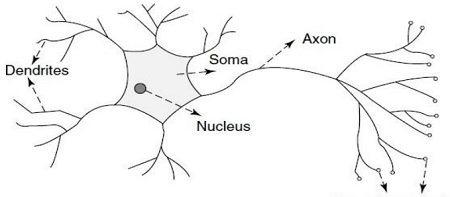
\includegraphics[scale=1.0]{bab2/gambar/selsaraf.jpg}}
    \end{center}
    \vspace{-20pt}
    \captionsetup{labelfont=bf, textfont=bf}
    \caption{Ilustrasi Sel Saraf}
    \vspace{-10pt}
    \captionsetup{labelfont=md, textfont=md}
    % \caption*{Sumber: https://upload.wikimedia.org/wikipedia/commons/b/b5/Neuron.svg}
    % \caption*{Sumber: Zhang (2019)}
    \label{fig:selsaraf}
\end{figure}

\section{Jaringan Saraf Tiruan}
\label{sec:2-JaringanSarafTiruan}

Jaringan Saraf Tiruan adalah sistem komputasi yang cara kerjanya menyerupai jaringan saraf pada otak
makhluk hidup.

layer, input, weight, output, inisialisasi

\section{Fungsi Aktivasi}
\label{sec:2-FungsiAktivasi}

sigmoid relu dkk

\section{Residual Network}
\label{sec:2-ResidualNetwork}

arsitektur resnet

\section{Optimisasi Arsitektur}
\label{sec:2-OptimisasiArsitektur}
lr, adam, loss function

\section{Estimasi Pose Dua Dimensi}
\label{sec:2-EstimasiPoseDuaDimensi}
citasi~\cite{8765346}

\section{Estimasi Pose Tiga Dimensi}
\label{sec:2-EstimasiPoseTigaDimensi}

citasi~\cite{martinez_2017_3dbaseline}

\section{PyTorch}
\label{sec:2-PyTorch}

pytorch dynamic graph

\begin{table}[htbp]
    \captionsetup{labelfont=bf, textfont=bf}
    \caption{Sebuah tabel}
    \vspace{-20pt}
    \begin{center}
        \begin{tabular}{| l c r |}
            \hline
            1 & 2 & 3 \\
            4 & 5 & 6 \\
            7 & 8 & 9 \\
            \hline
        \end{tabular}
    \end{center}
    \vspace{-10pt}
    \captionsetup{labelfont=md, textfont=md}
    \caption*{Sumber: Bego Lu}
\end{table}

